\chapter{Verfahren} \label{chap:training}

Das vierte Kapitel erläutert schrittweise das Verfahren zum Trainieren der EfficientNet-Modelle. Es beginnt mit der Beschreibung des Datenakquise-Prozesses. Anschließend wird detailliert auf die Verarbeitung der erworbenen Trainingsdaten mithilfe des MegaDetectors eingegangen. Im weiteren Verlauf betrachtet das Kapitel die Datenanalyse sowie Datenintegration in Einzelheiten und es schließt mit der Durchführung des Trainingsvorgangs.

\section{Datenakquise}

Zum Trainieren eines Klassifizierers benötigt man vor allem Trainingsdaten hoher Qualität. In Bezug auf das Projekt Natur 4.0 bedeutet dies, dass je mehr hochauflösende Bilder von den Tierarten im Marburger Universitätswald als Trainingsdaten benutzt werden, desto besser. Die Bilder von Natur 4.0 werden jedoch mit Kamerafallen aufgenommen, deren Qualität nicht immer gewährleistet ist. Wenn diese Bilder einem Klassifizierer übergeben werden, der zuvor nur mit hochwertigen Nicht-Kamerafallenbildern (abgekürzt: NK-Bildern) trainiert wurde, ist es möglich, dass der Klassifizierer solche Bilder aufgrund verrauschter Daten darin nicht gut klassifiziert, sogar nach der Verwendung des MegaDetectors. Dennoch sollte ein Klassifizierer so viele Merkmale wie möglich lernen, um die Klassen gut trennen zu können, was hauptsächlich durch Training mit Bildern hoher Qualität erreicht wird. Um dieses Dilemma aufzulösen, werden die EfficientNet-Modelle sowohl mit hochwertigen NK-Bildern als auch mit Kamerafallenbildern trainiert. Dazu müssen zunächst für jeden Typ entsprechende Datensätze gefunden werden.

\subsection{iNat}

%Der im \autoref{chap:relatedwork} besprochenen iNaturalist-Datensatz kommt von einer Datenquelle, deren Bilder von hoher Qualität sind. Diese Quelle ist die Webseite, die auch iNaturalist\footfullcite{iNatObservations} genannt wird, und zum Unterscheiden zwischen ihr und dem iNaturalist-Datensatz wird die Webseite im Weiteren als \emph{iNat} bezeichnet. 

Eine Datenquelle, deren Bilder von hoher Qualität sind, ist die Webseite iNaturalist\footfullcite{iNatObservations}. iNaturalist ermöglicht es Naturforschern, ihre visuellen Beobachtungen der Biodiversität weltweit zu teilen. Jede Beobachtung besteht aus einem Datum, Ort, Bildern (oder Video- sowie Audio-Dateien) und Beschriftungen, die den Namen und die \emph{Taxon-ID}\footnote{Unter dem Begriff \emph{Taxon} versteht man in der Biologie eine als systematische Einheit erkannte Gruppe von Lebewesen (z.~B. Stamm, Art). Die Taxon-ID ist eine eindeutige Nummer, die iNaturalist jedem Taxon zuordnet.} der im Bild vorkommenden Art enthalten. Es werden auch Anmerkungen zu dem beobachteten Tier sowie Qualitätsstufe der Bilder gespeichert. Zum Zeitpunkt dieser Arbeit hat die Webseite über 77 Mio. Beobachtungen von mehr als 345\,000 Arten gesammelt.

Da die Bilder von iNaturalist manuell und zielgerichtet aufgenommen wurden, liegt der Fokus jedes Bildes üblicherweise auf dem beobachteten Tier. Dies führt dazu, dass das Tier besser von seiner Umgebung unterscheidbar ist. Außerdem gibt es für jedes beobachtete Tier selten nur ein Bild, sondern üblicherweise mehrere Bilder aus verschiedenen Kamerawinkeln und somit mehr erlernbare Merkmale. Die Auflösungen von iNaturalist-Bildern sind allgemein im Vergleich zu Kamerafallenbildern höher, denn sie wurden meistens mit spezialisierten Kameras aufgenommen. Daneben sorgt das Evaluierungssystem der Webseite dafür, dass die Qualität der Bilder immer gewährleistet ist.

Der Datensatz, der aus gecrawlten iNaturalist-Bildern besteht, wird im weiteren Verlauf \emph{iNat} genannt. Im Folgenden wird der Prozess zum Anlegen von iNat beschrieben.

\begin{enumerate}
	\item Für das Projekt Natur 4.0 wurde eine Liste von 38 gewünschten Tierarten bereitgestellt (siehe \autoref{table:photosenseSpecies}), für die Bilder gecrawlt werden sollen. Zunächst ist dabei sicherzustellen, dass zwischen den Tierarten darin keine biologische Hierarchie besteht. Sonst kann es duplizierte Bilder bei mehreren Klassen in den Trainingsdaten geben, was die Gefahr von Overfitting erhöht und folglich zum Leistungsabfall des Klassifizierers führt. 
	
	Außerdem müssen die wissenschaftlichen Namen der aufgeführten Tierarten validiert werden. Dies geschieht, indem man nach ihren entsprechenden Taxon-IDs in iNaturalist sucht. Falls die Suche keine Ergebnisse oder duplizierte Taxon-IDs liefert, muss man Fehler in den Namen korrigieren oder gegebenenfalls die Namen entfernen, denn alle 38 aufgeführten Tierarten sind nach Biologen von Natur 4.0 in iNaturalist vorhanden und eindeutig identifiziert.
	
	\item Als Nächstes sind Bedingungen für die gecrawlten Bilder festzulegen. Jedes Bild soll über die höchste Qualitätsstufe Research-Grade nach iNaturalist-Standard verfügen. Daneben ist es erforderlich, dass die beobachteten Tiere als lebendig annotiert werden. Dies liegt daran, dass sich die Merkmale von Tierleichen stark von denen lebender Tiere unterscheiden können und letztlich nur lebende Tiere auf den Kamerafallenbildern erkannt werden sollen.
	
	\item Zum Schluss ist ein Crawler (zum Crawlen geschriebener Code) zu implementieren und auszuführen. Die Funktionsweise des Crawlers ist wie folgt: Zuerst holt er alle Beobachtungen einer der gegebenen Tierarten.	Danach lädt der Crawler die Bilder dieser Tierart herunter, indem er die URLs verwendet, die sich in jeder geholten Beobachtung befinden. Diese Vorgehensweise wird im weiteren Verlauf für jede Tierart in der gegebenen Liste wiederholt. 
	
	Im Crawler erfolgt das Holen von Beobachtungen durch die Verwendung der \emph{iNaturalist-API}\footfullcite{iNatAPI} und des \emph{pyinaturalist-Moduls}\footfullcite{pyinat}. Die Schnittstelle iNaturalist-API bietet eine Reihe von Methoden wie \code{create}, \code{delete}, \code{update}, \code{search} und \code{fetch} zum Interagieren mit den Biodiversitätsdaten der iNaturalist-Webseite durch Anfragen und Antworten. Das pyinaturalist-Modul ermöglicht es, auf diese Methoden der API über die Programmiersprache Python zuzugreifen.
	
	
\end{enumerate}

Nach dem Crawlen von iNaturalist-Bildern treten zwei Probleme auf.

\begin{enumerate}
	\item Die Bildanzahl der Tierarten ist stark ungleichmäßig verteilt. Während das Minimum 25 ist, beträgt das Maximum 8406 (mehr als 300-mal größer). Wenn alle gecrawlten iNaturalist-Bilder z.~B. in einen Klassifizierer eingespeist werden, um ihn zu trainieren, ist es gut möglich, dass der Klassifizierer die Merkmale der Tierarten mit kleinerer Bildanzahl ignoriert und sich nur an die Arten mit größerer Anzahl von Bilder anpasst. Dieses Problem nennt man \emph{Imbalanced Classification} und es lässt sich dadurch teilweise behandeln, dass man bei der Datenakquise eine Obergrenze für die Anzahl der zu crawlenden Bilder festsetzt (Mehr Lösungsansätze dazu in \autoref{sec:dataintegration} und \autoref{sec:evalmetrics}).

	\item Unter den heruntergeladenen Bildern befinden sich solche mit nur tierischen Fußabdrücken oder Exkrementen. Ein denkbarer Lösungsansatz dafür ist die Verwendung der iNaturalist-API sowie des pyinaturalist-Moduls zur Filterung dieser unerwünschten Beobachtungen. Allerdings ist eine Methode dazu in der API noch nicht verfügbar. Eine weitere Lösung besteht darin, eine solche Methode selbst zu schreiben. Trotzdem erweist sich dieser Ansatz als höchst aufwändig. Es gibt in keiner iNaturalist-Beobachtung Beschriftungen, die markieren, dass die Bilder Tierpfoten sowie Tierkote enthalten. Daneben erfordert das Training eines Modells zum Erkennen von tierischen Fußspuren und Exkrementen möglicherweise genauso viel Kosten wie das Training eines Modells zur Tierarterkennung.
	
	Die Bilder mit Tierpfoten sowie Tierkots können den Klassifizierer während des Trainings negativ beeinflussen, jedoch ist der Leistungsabfall geringfügig, denn diese Bilder machen nur einen winzigen Anteil der gecrawlten Bilder aus. Deshalb kann man dieses Problem überspringen.
\end{enumerate}

\subsection{Nat4 und WCS}

Als mögliche Quellen für Kamerafallenbilder bieten sich sowohl das Forschungsprojekt \emph{Langfristige Populationsentwicklung krankheitsübertragender Nagetiere} (abgekürzt: Nagetier) \cite{imholt2021langfristige} als auch das \emph{Snapshot-Wisconsin-Projekt}\footfullcite{snapshotWCS} (abgekürzt: Wisconsin) an. In den beiden Projekten wurden Tierbilder ausschließlich von Kamerafallen aufgenommen. Während Nagetier 63\,789 Bilder von 20 Säugetierarten gesammelt hat, verfügt Wisconsin über mehr als 3 Mio. Bilder von 43 Tierarten. Wie bei iNaturalist wird jedem Nagetier- bzw. Wisconsin-Bild eine eindeutige ID zugewiesen.

Im Vergleich zu iNaturalist-Bildern sind Kamerafallenbilder in der Regel von niedrigerer Qualitätsstufe. Die Kamerafallen werden an festen Positionen aufgestellt, was dazu führt, dass die Bilder nur aus einer begrenzten Anzahl von Kamerawinkeln aufgenommen werden können. Da die Kamerafallen wärme- bzw. bewegungsaktiviert sind, liegt der Fokus jedes Bildes meistens nicht auf dem beobachteten Tier, d.~h. es wird schwieriger, das Tier von seiner Umgebung zu unterscheiden.

Die Datensätze, die sich aus dem Crawlen der Bilder von den Projekten Nagetier und Wisconsin ergeben, werden jeweils als \emph{Nat4} und \emph{WCS} bezeichnet. Der Nat4-Datensatz wurde zuvor gecrawlt und von dem Projekt Natur 4.0 zur Verfügung gestellt (daher der Name). Der Grund, warum Wisconsin-Bilder nach Bereitstellung des Nat4-Datensatzes noch benötigt werden, liegt darin, dass nur beide Datensätze zusammen die meisten der gewünschten Tierarten in \autoref{table:photosenseSpecies} abdecken können. Im Folgenden wird der Prozess zum Crawlen von Bildern für den Datensatz WCS beschrieben.

\begin{enumerate}
	\item Zunächst ist zu bestimmen, von welchen Tierarten die Bilder gecrawlt werden. Die Datenbank des Wisconsin-Projekts verfügt aber nicht über alle Tierarten in \autoref{table:photosenseSpecies}. Es lassen sich nur 14 davon finden.
	
	\item Als Nächstes müssen Bedingungen für die gecrawlten Bilder festgelegt werden. Jedoch im Gegensatz zu iNaturalist wird von Wisconsin keine API bereitgestellt, die die Filterung der Kamerafallenbilder ermöglichen. Darüber hinaus sind die für iNaturalist-Bilder geltenden Bedingungen beim Wisconsin-Projekt entweder nicht anwendbar oder wurden  bereits erfüllt. Es gibt in Wisconsin kein Evaluierungssystem, sodass man die Bilder in Bezug auf ihre Qualitätsstufen suchen kann. Da die Kamerafallen nur wärme- und bewegungsaktiviert sind, ist es unmöglich, dass Tierleichen in den Bildern aufgezeichnet werden. 
	
	Trotz der Nichtverfügbarkeit einer API in Wisconsin zur Filterung der Bilder ist es möglich (und auch empfehlenswert), eine maximale Anzahl der zu crawlenden Bilder für jede Tierart vorzudefinieren, um das Imbalanced-Classification-Problem vorab möglichst zu vermeiden. %Konkret wird dieses Maximum für alle Arten auf 2000 festgelegt.
	
	\item Der letzte Schritt ist die Implementierung und Ausführung eines Crawlers zum Herunterladen von Bildern aus dem Wisconsin-Projekt. Damit ein Download-Link für jedes Bild generiert werden kann, sind zuerst die jeder Tierart zugehörigen Bilder bzw. Bild-IDs zu bestimmen.	Man muss aber die IDs in externen Archiven suchen, weil keine API von Wisconsin zur Verfügung gestellt wird. Für diese Arbeit wurde der Datensatz \emph{Snapshot-Wisconsin-Images}\footnote{Es stellt sich die Frage, warum die Bilder des Datensatzes Snapshot-Wisconsin-Images nicht als Trainingsdaten verwendet werden. Das Problem ist, dass diese Bilder eine stark reduzierte Auflösung (nur 330$\times$330 Pixel) haben, weshalb es nötig ist, mit dem Crawlen von Wisconsin-Bildern in der Originalauflösung fortzufahren.} \cite{WCSOrigin}, der sich aus fast 0,5 Mio. Wisconsin-Bildern zusammensetzt, als die Quelle für die IDs verwendet. Die Bilder darin sind ordnerweise nach Tierart gruppiert und mit den IDs benannt, unter denen sie auch auf der Snapshot-Wisconsin-Website\footfullcite{WCSBaseURL} zu finden sind. Solche Bild-IDs werden extrahiert und anschließend vom Crawler mit der (Basis-)URL dieser Website verknüpft, damit der Crawler Download-Links erstellen und die entsprechenden Wisconsin-Bilder herunterladen kann.
	
\end{enumerate}

%Es ist nötig, die maximale Anzahl der zu crawlenden Bilder jeder Tierart vorzudefinieren, um das Problem der ausgewogenen Klassifizierung möglichst zu vermeiden.

Die erworbenen Bilder werden je nach Tierart in verschiedenen Ordner gelegt, die nach den wissenschaftlichen Namen der Tierarten genannt sind.

\section{MegaDetecting}

Wie bereits in \autoref{sec:megadetector} gezeigt dient der MegaDetector zur Vereinfachung der Klassifizierung von lokalisierten Tieren, indem die unnötigen Pixel entfernt werden (siehe \autoref{fig:MegadetectorRedFox}). Auf genau die gleiche Weise erfolgt die Verarbeitung der erworbenen Trainingsdaten, d.~h. es werden für die Klassifizierer nur die Bounding Boxes von den lokalisierten Tieren als Trainingsdaten verwendet. Dadurch lernen die Klassifizierer keine redundanten Merkmale, sondern nur solche, die für die Klassifizierung von Tierarten erheblich sind.

Im Folgenden wird beschrieben, wie man mittels des MegaDetectors die Bounding Boxes als Trainingsdaten für die EfficientNet-Modelle gewinnen kann. Der Gesamtprozess wird \emph{MegaDetecting} genannt und erfolgt in zwei Schritten.

\begin{enumerate}

	\item Der erste Schritt ist die Lokalisierung von Tieren, d.~h. die Anwendung des MegaDetectors auf die erworbenen iNat-, Nat4- und WCS-Bilder.	Dabei wird für jede Tierart in jedem Datensatz eine JSON-Datei erstellt, die die Koordinaten der auszuschneidenden Bounding Boxes enthält (siehe \autoref{fig:jsonMegaDetect}).
	
	\item Der zweite Schritt besteht darin, die Bounding Boxes aus den erworbenen Bildern auszuschneiden. Obwohl es mehrere MegaDetections pro Bild geben kann, wird zur Vermeidung von Overfitting lediglich der Bounding Box ausgeschnitten, der der MegaDetection mit dem größten Confidence-Wert entspricht. Zusätzlich muss dieser Confidence-Wert größer als 0,8 sein, damit die MegaDetection als vertrauenswürdig angesehen werden kann. Beispielsweise in \autoref{fig:jsonMegaDetect} wird die zweite MegaDetection nicht verwendet, weil ihr Confidence-Wert weder am größten noch größer als 0,8 ist. Die Schwellenwertauswahl von 0,8 basiert darauf, dass 0,8 der Standardwert im MegaDetector für zuverlässige Lokalisierungsergebnisse ist. 
	
	\begin{figure}[h]
		\centering
		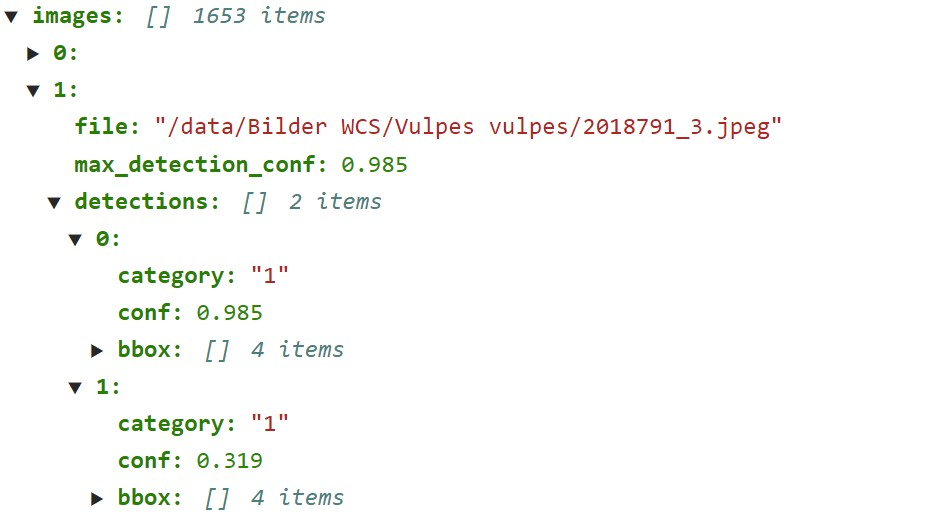
\includegraphics[width=0.95\linewidth]{images/jsonMegaDetect}
		\caption{Ausschnitt aus der JSON-Datei, die aus der Anwendung des MegaDetector auf Bilder der Tierart ''Vulpes vulpes'' im WCS-Datensatz resultiert. In jeder ''detection'' (MegaDetection) verweist ''bbox'' auf die Koordinaten der Bounding Boxes lokalisierter Tiere, während ''conf'' die entsprechenden Confidence-Werte der Lokalisierung bezeichnet. Die MegaDetections werden nach Confidence-Wert absteigend aufgelistet.}
		\label{fig:jsonMegaDetect}
	\end{figure}
	
	Falls zwei oder mehrere MegaDetections von demselben Bild den gleichen größten Confidence-Wert haben, der zugleich größer als 0,8 ist, kommt der Einfachheit halber nur die erst aufgeführte MegaDetection zum Einsatz. Als bessere aber aufwändigere Alternativen kann man alle solchen MegaDetections oder nur diejenige benutzen, die der größten Bounding Box entspricht. Jedoch kommt dieser Fall selten vor und somit sind keine komplizierten Implementierungen erforderlich.
\end{enumerate}


\section{Datenanalyse und Datenintegration} \label{sec:dataintegration}

Da die EfficientNet-Modelle sowohl mit hochwertigen NK-Bildern als auch mit Kamerafallenbildern trainiert werden, gelten als ihre Trainingsdaten nur die Bilder von den Tierarten, die sowohl in iNat als auch in Nat4 und WCS vorkommen. Es ist ebenso wichtig, dass jede von solchen Tierarten über genügende Trainingsbilder (ausgeschnittene Bounding Boxes) verfügt, damit sich die Gefahr von \emph{Underfitting}\footnote{Der Begriff verweist auf einen Effekt, der auftritt, wenn ein zu einfaches Modell neue Daten nicht gut vorhersagt, weil es den Zusammenhang zwischen den Einflussvariablen und der Zielvariable aufgrund der unzureichenden Komplexität nicht erkennt \cite{Novustat}.} verringern lässt und es ausreichende Daten zum Testen der Klassifizierer gibt. Gemäß \cite[13]{SHAHINFAR2020101085} ist die empfohlene minimale Anzahl 150 Bilder pro Klasse. Tierarten, die diese Bedingung erfüllen, werden in \autoref{table:MDcount} mit ihrer entsprechenden Trainingsbilderanzahl aufgelistet.

%also es soll durchschnittlich mindestens 75 Trainingsbilder pro Tierart jedes Bildertyps geben. Das Problem ist aber, dass man danach nur noch 18 Arten hat, weniger als 50\% der zu klassifizierenden Tierarten in \autoref{table:photosenseSpecies}. Daher wird das Minimum für jeden Bildertyp auf 50 Trainingsbilder pro Tierart gesetzt. 

\begin{table}[h]
	\centering
	\caption{Anzahl von Trainingsbilder jeder Tierart in iNat sowie Nat4 \& WCS (nach Gesamtzahl aufsteigend sortiert)}
	\label{table:MDcount}
	\begin{tabular}{l|>{\raggedright}m{3cm}|r|>{\raggedleft}m{1.6cm}|r}
		\textbf{Tierart}     & \textbf{Deutscher Name}          & \textbf{Gesamt} & \textbf{iNat} & \textbf{Nat4 \& WCS} \\
		\hline
		Martes martes    & Baummarder     & 174    & 110  & 64          \\
		Mustela nivalis  & Mauswiesel      & 228    & 145  & 83          \\
		Castor fiber     & Biber     & 317    & 199  & 118         \\
		Felis silvestris & Wildkatze     & 360    & 83   & 277         \\
		\hline
		Lutra lutra      & Fischotter     & 687    & 133  & 554         \\		
		Canis lupus      & Wolf     & 718    & 300  & 418         \\
		Cervus elaphus   & Rothirsch     & 836    & 694  & 142         \\
		Meles meles      & Dachs     & 1325   & 276  & 1049        \\
		\hline
		Dama dama        & Damhirsch     & 1464   & 294  & 1170        \\
		Ursus arctos     & Braunbaer     & 2252   & 302  & 1950        \\
		Felis catus      & Hauskatze     & 2360   & 1908 & 452         \\
		Lepus europaeus  & Feldhase     & 2727   & 698  & 2029        \\
		\hline
		Sciurus vulgaris & Europaeisches Eichhoernchen     & 3656   & 3281 & 375         \\
		\hline
		Sus scrofa       & Wildschwein     & 4047   & 1046 & 3001        \\
		Oryctolagus cuniculus & Wildkaninchen & 5268   & 604  & 4664        \\
		Alces alces      & Elch     & 6975   & 1403 & 5572        \\
		Vulpes vulpes    & Fuchs     & 9455   & 4719 & 4736        \\
		\hline
		Procyon lotor    & Waschbaer     & 11870  & 3326 & 8544        \\
		Capreolus capreolus & Europaeisches Reh  & 16635  & 2251 & 14384      
	\end{tabular}
\end{table}

Aus \autoref{table:MDcount} kann man sehen, dass die Gefahr des Imbalanced-Classification-Problems trotz Beschränkung der Anzahl der zu crawlenden Bilder noch groß ist. Dies liegt daran, dass der gecrawlte iNat- und der bereitgestellte Nat4-Datensatz wesentlich unausgewogen sind. Zur Behandlung dieses Problems kann man zusätzlich die Anzahl der zum Trainieren verwendeten Bilder begrenzen. Wird diese Zahl beispielsweise auf 200 beschränkt, bedeutet dies, dass während einer Trainingsepoche maximal 200 zufällig ausgewählte Bilder pro Tierart zum Trainieren der Klassifizierer verwendet werden dürfen. Da jede Art in \autoref{table:MDcount} insgesamt mindestens 100 Trainingsbilder hat, kann man zum Trainieren der EfficientNet-Modelle bis zu 500 Bilder pro Tierart benutzen, ohne weitere Maßnahmen gegen das Imbalanced-Classification-Problem zu ergreifen.

Die gesamten Daten der in \autoref{table:MDcount} aufgeführten Tierarten werden in Training-, Validierung- sowie Testdatensatz unterteilt, um das beste EfficientNet-Modell zur Klassifizierung dieser Tierarten zu finden (mehr dazu in \autoref{sec:modelltraining}). Die Aufteilung erfolgt im Verhältnis 70\% für das Training, 10\% für die Validierung und 20\% für das Testen (siehe \autoref{table:splitcount}). Damit soll sichergestellt werden, dass es sogar bei der Tierart mit der kleinsten Bildanzahl hinreichende Trainingsbilder zum Testen der Klassifizierer gibt, d.~h. die zugeteilten Testbilder sind in der Lage, Abweichungen in den visuellen Daten dieser Tierart abzudecken und darzustellen, wie sie allgemein aussieht.

\begin{table}[h]
	\centering
	\caption{Trainingsbilderanzahl in jedem aufgeteilten Datensatz.}
	\label{table:splitcount}
	\begin{tabular}{l|r|r|r}
		\textbf{Datensatz}   & \textbf{Gesamt} & \textbf{iNat}  & \textbf{Nat4 \& WCS} \\
		\hline
		Training    & 49924  & 15230 & 34694       \\
		Validierung & 7131   & 2174  & 4957        \\
		Test        & 14292  & 4363  & 9929       
	\end{tabular}
\end{table}

\section{Modelltraining} \label{sec:modelltraining}

Vor der Durchführung des realen Trainingsvorgangs soll festgelegt werden, welche von den EfficientNet-Modellen zu trainieren sind. Es gibt insgesamt acht EfficientNet-Modelle von B0 bis B7 und damit sich Zeit und Ressourcen für das Training dieser Modelle sparen lassen, empfiehlt es sich, die Anzahl der zu trainierenden Modelle einzuschränken. Auf der einen Seite sind hinsichtlich der Top-1-Accuracy die tieferen Modelle besser, aber ihr Training dauert länger und die dafür benötigte Anzahl der FLOPs sowie die Parameteranzahl sind auch größer. Auf der anderen Seite erreichen die flacheren EfficientNet-Modelle eine niedrigere Top-1-Accuracy, dennoch ist die Dauer ihres Trainings kürzer und die von ihnen benötigte Anzahl der FLOPs sowie die Parameteranzahl sind kleiner. Da letztlich die Accuracy als wesentlicher als die Kosten des Trainings gilt, werden die Modelle B3 bis B7 zum Trainieren ausgewählt. Ein weiterer Grund dafür liegt darin, dass die Trainingsbilder über eine Median-Auflösung von 265$\times$299 Pixel verfügen, die der Eingabeauflösung des B3-Modells (300$\times$300)\footfullcite{EffNetBaseModelResolution} entspricht. Dies bedeutet, dass wenn die Modelle B0, B1 und B2 mit kleineren Eingabeauflösungen (224$\times$224, 240$\times$240 bzw. 260$\times$260) zum Trainieren verwendet werden, werden mehr als 50\% der Trainingsbilder geschrumpft, was zum Verlust von möglicherweise wertvollen Merkmalen in den visuellen Daten führen kann.

Es wird lediglich ein Modell zur Tierklassifizierung benötigt. Dieses wird bestimmt, indem zuerst jedes potenzielle EfficientNet-Modell für eine vordefinierte Anzahl von Trainingsepochen auf dem Trainingsdatensatz trainiert wird. Nach jeder Epoche wird das trainierte Modell auf dem Validierungdatensatz evaluiert, um zu prüfen, ob es verbessert wird. Falls ja, wird diese bessere Version des Modells gespeichert. Zum Schluss werden die besten Versionen aller EfficientNet-Modelle hinsichtlich ihrer Leistungen auf dem Testdatensatz verglichen, um daraus das beste trainierte Modell zur Tierklassifizierung auszuwählen.

Das Training der EfficientNet-Modelle erfolgt in fünf Schritten.

\begin{enumerate}
	\item \textbf{Datenaugmentierung}
	
	Bevor die Daten in das Modell eingespeist werden, werden sie augmentiert. Das bedeutet, dass die Trainingsbilder zufällig leicht gedreht, verschoben, gespiegelt werden und ihr Kontrast angepasst wird. Durch das Erstellen modifizierter Versionen von Bildern im Trainingsdatensatz trägt dieser Schritt dazu bei, weitere mögliche Abweichungen in den visuellen Daten der Tierarten abzudecken und somit die Gefahr von Overfitting während des Trainings zu verringern \cite{Shorten2019}.
	
	\item \textbf{Initialisierung}
	
	Bei diesem Schritt wird das zu trainierende EfficientNet-Modell mit den vortrainierten ImageNet-Gewichten initialisiert. Da dieses Modell zuvor zur Klassifizierung tausend Klassen verwendet wurde, gibt seine Ausgabeschicht einen eindimensionalen Vektor der Größe 1000 aus (siehe \autoref{fig:imgKlassifizierungProzess}), der mit den 19 zu klassifizierenden Tierarten in \autoref{table:MDcount} inkompatibel und daher zu entfernen ist. Nach der Entfernung werden neue trainierbare Schichten zum Modell hinzugefügt, welche die gleichen Eingaben für die alte Ausgabeschicht aufnehmen und in Klassifizierungsergebnisse der erworbenen Tierbilder transformieren.
	
	\item \textbf{Einfrierung des vortrainierten Modells}
	
	Der nächste Schritt ist das Einfrieren des vortrainierten Teils des Modells, d.~h. die vortrainierten Gewichte werden als konstant gesetzt. Falls diese Gewichte während des Trainings abgeändert werden, wird alles verloren, was bereits von dem ImageNet-Datensatz gelernt wurde. Dies ist nicht anders, als das Modell von Grund auf neu zu trainieren.
	
	\item \textbf{Transfer Learning}
	
	Das gesamte Modell lässt sich nun gleichzeitig auf dem Trainingsdatensatz trainieren und auf dem Validierungdatensatz evaluieren. Während dieses Prozesses werden lediglich die Gewichte der neuen hinzugefügten Schichten optimiert und die Top-1 bzw. Top-5 Accuracy (Leistungen) sowie der \emph{Cross-Entropy Loss}\footfullcite{CrossEntropyLoss} (Kosten) des Modells auf dem Validierungdatensatz erfasst. Die Validierungkosten werden verwendet, um zu testen, ob das Modell nach einer Trainingsepoche verbessert wird oder nicht (Je niedriger, desto besser). Wenn der erstere Fall passiert, werden die ihm entsprechenden Gewichte abgespeichert.
	
	\item \textbf{Verbesserung des Modells durch Feintuning}
	
	Nach dem Transfer Learning kann man die Leistung des trainierten Modells erhöhen, indem man zuerst seine vortrainierten Schichten ''auftaut'', d.~h. man setzt die bisher als konstant gesetzten Gewichte wieder als änderbar. Danach wird das aufgetaute Modell nochmals auf dem Training- und Validierungdatensatz trainiert bzw. evaluiert. Dabei ist zu beachten, dass die \emph{Lernrate} (Optimierungsrate der Gewichte) klein gewählt wird, sonst kann es zu Overfitting führen.
\end{enumerate}

Die detaillierten Trainingskonfigurationen der EfficientNet-Modelle sowie ihre Leistung auf dem Testdatensatz werden in \autoref{chap:experimentresult} gezeigt.

